\documentclass[tikz]{standalone}

%%%%%%%%%%%%%%%%%%%%%%%%%%%%%%%%
% black 
\definecolor{rbrown}{HTML}{996633}
\definecolor{rred}{HTML}{FF0000}
\definecolor{rorange}{HTML}{FF9900}
\definecolor{ryellow}{HTML}{FFFF00}
\definecolor{rgreen}{HTML}{228b22}
\definecolor{rblue}{HTML}{0047AB}
\definecolor{rviolet}{HTML}{800080}
\definecolor{rgrey}{HTML}{CCCCCC}
\definecolor{rwhite}{HTML}{FFFFFF}
\definecolor{kulta}{HTML}{FFD700}
\definecolor{hopea}{HTML}{C0C0C0}
\definecolor{lightb}{HTML}{ADD8E6}
\definecolor{sand}{HTML}{C2B280}
%%%%%%%%%%%%%%%%%%%%%%%%%%%%%%%
\begin{document}
\newcommand\Stripe[2]{\draw[fill=#2,#2] ++(#1,0) +(-0.15,-0.71) rectangle +(0.15,0.71);}
% \stripe{offset}{color} short stripe
\newcommand\stripe[2]{\draw[fill=#2,#2] ++(#1,0) +(-0.15,-0.51) rectangle +(0.15,0.51);}

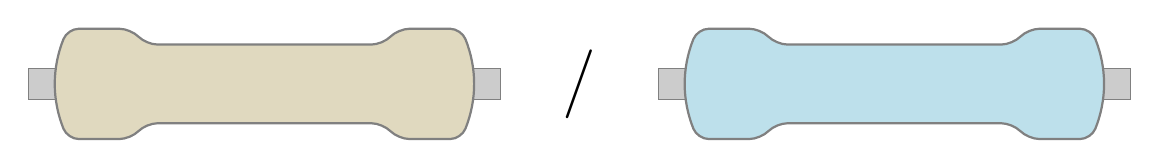
\begin{tikzpicture}
  % wire
  \draw[gray,fill=gray!40] (-3,-0.2) rectangle (3,0.2);
  % resistor
  \draw[rounded corners,thick,gray,fill=sand!50]
  ++(0,0.5) -- ++(1.5,0) -- ++(0.2,0.2) -- ++(0.8,0)
  .. controls +(0.2,-0.5) and +(0.2,0.5) .. ++(0,-1.4) -- ++(-0.8,0)
  -- ++(-0.2,0.2) -- ++(-3,0) -- ++(-0.2,-0.2) -- ++(-0.8,0)
  .. controls +(-0.2,0.5) and +(-0.2,-0.5) .. ++(0,1.4) -- ++(0.8,0)
  -- ++(0.2,-0.2) -- cycle;
  \Stripe{-2.1}{rred}
 \stripe{-1.2}{rred}
  \stripe{0.2}{rbrown}
    \Stripe{2.1}{kulta}
    
    \node at (4,0) {\Huge{$/$}};
  \begin{scope}[shift={(8,0)}]
    % wire
  \draw[gray,fill=gray!40] (-3,-0.2) rectangle (3,0.2);
  % resistor
  \draw[rounded corners,thick,gray,fill=lightb!80]
  ++(0,0.5) -- ++(1.5,0) -- ++(0.2,0.2) -- ++(0.8,0)
  .. controls +(0.2,-0.5) and +(0.2,0.5) .. ++(0,-1.4) -- ++(-0.8,0)
  -- ++(-0.2,0.2) -- ++(-3,0) -- ++(-0.2,-0.2) -- ++(-0.8,0)
  .. controls +(-0.2,0.5) and +(-0.2,-0.5) .. ++(0,1.4) -- ++(0.8,0)
  -- ++(0.2,-0.2) -- cycle;
  \Stripe{-2.1}{rred}
  \stripe{-1.2}{rred}
  \stripe{-0.2}{black}
  \stripe{1.2}{black}
 \Stripe{2.1}{kulta}
  \end{scope}
\end{tikzpicture}
\end{document}